\documentclass[12pt,a4paper,]{scrreprt}
\usepackage[ngerman]{babel}
\usepackage[onehalfspacing]{setspace}
\usepackage[utf8]{inputenc}
\usepackage{graphicx}
\usepackage{array}
\usepackage{gnuplottex}
\usepackage{siunitx}

\usepackage{multicol}
\usepackage{capt-of}
\usepackage{amsmath}
\usepackage{ulem}
\usepackage{amsthm}

\setkomafont{chapter}{\fontsize{20bp}{22.2bp}\selectfont\bfseries}
\setkomafont{chapter}{\fontsize{14bp}{18.8bp}\selectfont\bfseries}
\setkomafont{section}{\fontsize{12bp}{14.4bp}\selectfont\bfseries}
\renewcommand{\chapterheadstartvskip}{\vspace*{-1\topskip}}
\renewcommand{\chapterheadendvskip}{\vspace*{0.8\topskip}}
%---------------------------------------------------------------------------------------------------------------------------------------------------------------
% Ende der Einstellungen
%---------------------------------------------------------------------------------------------------------------------------------------------------------------

%---------------------------------------------------------------------------------------------------------------------------------------------------------------
%Ab hier gibt es Inhalt
%---------------------------------------------------------------------------------------------------------------------------------------------------------------
\begin{document}

	\title{Erzwungene Schwingungen\\(Korrektur)} 
	\author{Henrik Jäger \\ 3114168 \and Lena Majer \\ 3115808}
	\subtitle{M30a \\  Assistent: Michael Zimmer}
	\subject{Physikalisches Praktikum I}
	\publishers{Universität Stuttgart}
	%\thanks{Assistent: Sascha Kolatschek}

	\maketitle% Titelei

	\tableofcontents   %Inhaltsverzeichnis

	\pagebreak
    
	\chapter{Versuchsbeschreibung}
  
    
		\section{Ziel}
			In diesem Versuchstag geht es um die Bestimmung der Amplitude von gedämpften, ungedämpften und getriebenen Schwingungen. Zudem soll die Eigenfrequenz bestimmt werden. Als Messgerät wird ein Drehschwinger verwendet.
		
        \section{Grundlagen}
			Als Grundlage zu diesem Versuchstag sind vorallem die Differentialgleichungen der jeweiligen Schwingungen zu betrachten. \\
			Für die ungedämpfte harmonische Schwingung gilt:\\
			\begin{equation}
				J \cdot \ddot \Psi + D \cdot \Psi = 0
			\end{equation}
			Die Lösung hierfür lautet:\\
			\begin{equation}
				\Psi = a \cdot e^{i \cdot \omega_0 \cdot t} + b \cdot e^{-i \cdot \omega_0 \cdot t}
			\end{equation}
			a und b sind Konstanten und $\omega_0$ wird beschrieben durch
			\begin{equation}
				\omega_0=\frac{2\pi}{T_0}
			\end{equation}
			Für die gedämpfte harmonische Schwingung gilt:\\
			\begin{equation}
				J \cdot \ddot \Psi + B \cdot \dot \Psi + D \cdot \Psi = 0
			\end{equation}
			Mit der Lösung:\\
			\begin{equation}
				\Psi = e^{\frac{-B}{2J}t}\cdot (\alpha e^{ \sqrt{\frac{B^2}{4J^2}-\frac{D}{J}}\cdot t}+\beta e^{ -  \sqrt{\frac{B^2}{4J^2}-\frac{D}{J}}\cdot t})
			\end{equation}
			Und 
			\begin{equation}
				\omega=\frac{2\pi}{T_1}=\sqrt{\frac{B^2}{4J^2} - \frac{D}{J}}
			\end{equation}
			Für die erzwungene  Schwingung gilt:\\
			\begin{equation}
				J \cdot \ddot \Psi + B \cdot \dot \Psi + D \cdot \Psi = M_0 \cdot cos(\omega \cdot t)
			\end{equation}
			Und der Lösung:\\
			\begin{equation}
				\Psi =\frac{M_0}{\sqrt{I^2 \cdot (\omega_0^2- \omega^2)^2+B^2 \cdot \omega^2}} \cdot cos(\omega \cdot t-\Phi)
			\end{equation}
			Mit:\\
            \begin{equation}
				\Phi = \text{arctan}(\frac{B \cdot \omega}{I \cdot \omega_0^2 \cdot \omega^2})
			\end{equation}
Die Richtgröße der Spiralfeder wird mit D beschrieben. I beschreibt das Trägheitsmoment. $\omega$ beschreibt die Kreisfrequenz. $\Psi$ beschreibt die Amplitude der Schwingung.

			\pagebreak
	
    
    
    
    
    
    
    
    
    
	\chapter{Messprinzip mit Skizze und Versuchsablauf}
    
      \begin{center}
    
    	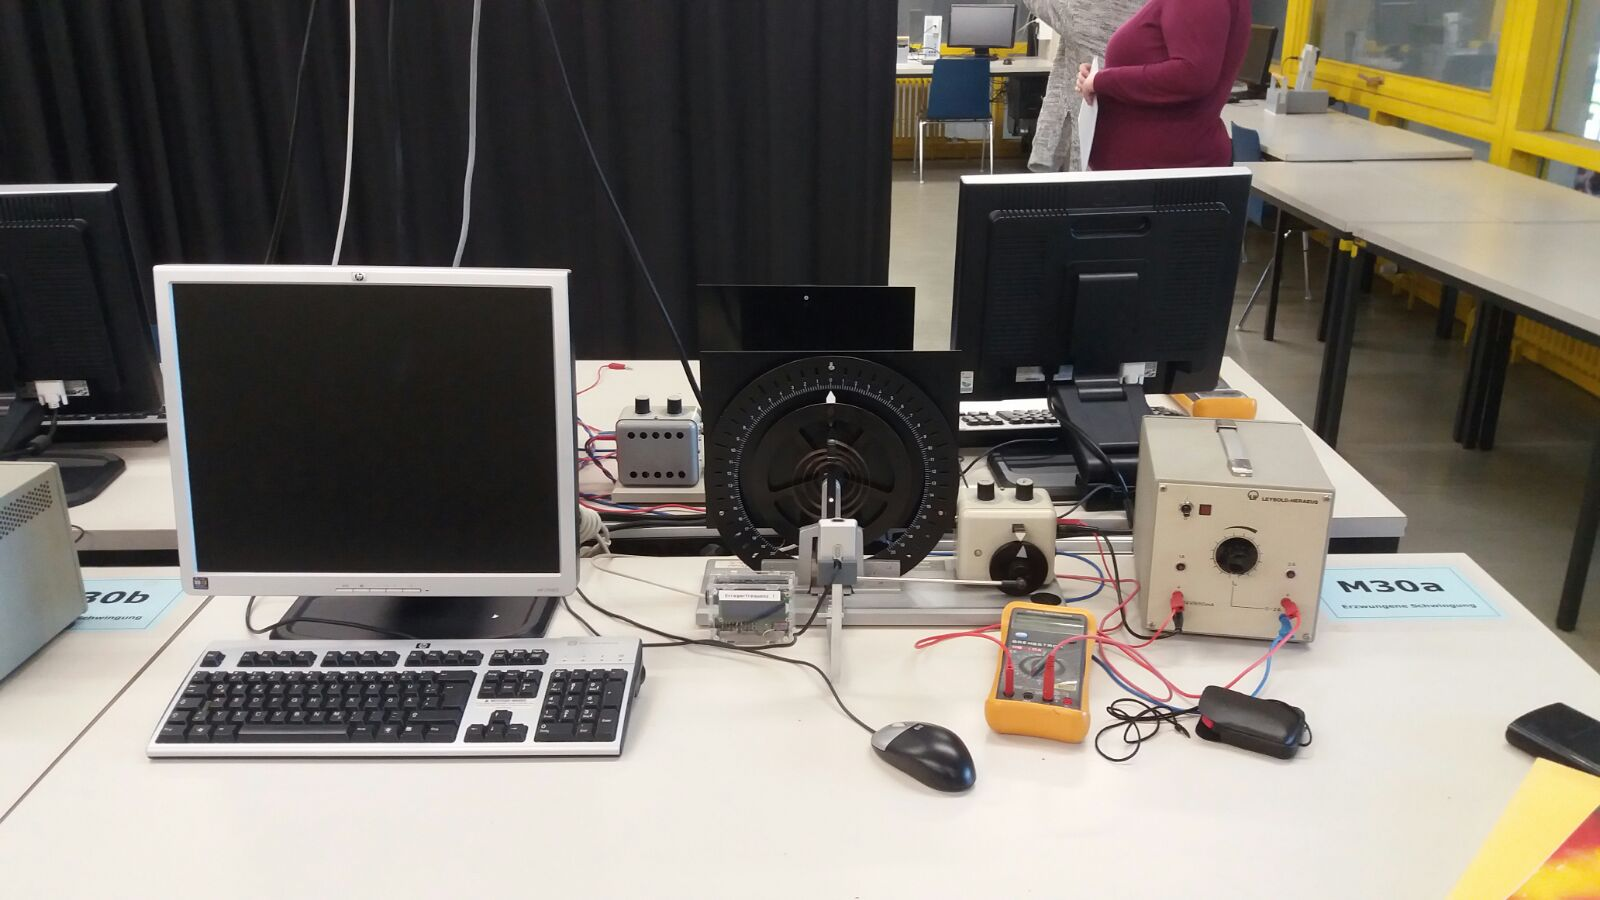
\includegraphics[scale=0.25]{Unknown.jpg}
        \captionof{figure}[]{Versuchsaufbau}
        \end{center}
		\section{1.Aufgabenteil:}
			Im ersten Aufgabenteil wird die Zeit von 10 Perioden des ungedämpfen System bestimmt. Aus diesen Messdaten kann die Eigenfrequenz dieses schwingenden Systems bestimmt werden.\\
		
        
        \section{2.Aufgabenteil:}
			Im folgenden Aufgabenteil wird wiederum die Schwingdauer von 10 Perioden eines schwingendes Systems bestimmt. Jedoch wird hierbei eine Dämpfung eingeschalten. Dabei handelt es sich um eine Wirbelstrombremse. 			Diese Messung wird bei 0,2A und 0,4A durchgeführt. Aus dem Ergebnis kann zu jeder Dämpfung die jeweilige Eigenfrequenz bestimmt werden. \\
		
        
        \section{3.Aufgabenteil:}
			Im dritten Aufgabenteil geht es um die Bestimmung des logarithmischen Dekrements und der Abklingkonstante. Mithilfe einer Kamera werden die gedämpften Schwingungen aufgezeichnet mit einem Computerprogramm die Amplituden in Abhängigkeit der Zeit gemessen. Hiermit werden die gesuchten Werte bestimmt. Die Schwingung wird für 0,2 A und 0,4 A - Wirbelstrombremse - über eine Kamara aufgezeichnet. Über das Computersystem wird das Aufgenommene ausgewertet. Durch die Auswertung können die gesuchten Daten ermittelt werden. \\
		
        
        \section{4.Aufgabenteil:}
			Im vierten Aufgabenteil geht es um die weitere Auswertung der bereits getätigten Messungen. Hierbei soll quantitativ das Verhalten von gedämpfter und ungedämpfter Schwingung verglichen werden.\\
		
        
        \section{5.Aufgabenteil:}
			Im letzten Teil geht es um eine getriebe Schwingung. Dazu wird ein Motor verwendet, der das System treibt. Hierbei soll eine Resonanzkurve bestimmt werden. Dabei wird bei verschiedenen Frequenzen, um die Resonanzfrequenz,  die Amplitude und die Zeit von 10  Perioden bestimmt. Um diese bestimmen zu können, muss abgewartet werden, bis der Einschwingvorgang vorbei ist. Erst danach kann gemessen werden. 

		\pagebreak
	
    
    
    
    
    
    
    
    
    
    
    
    
    
    
    
    \chapter{Formeln}
Die Kreisfrequenz $\omega$ kann über die Periodendauer bestimmt werden:
		\begin{equation}
			\omega = \frac{2\pi}{T}
		\end{equation}
        (T: Periodendauer) \\
	Das loarithmische Dekrement $\Lambda$ lässt sich bestimmen durch:
 
		\begin{equation}
			\Lambda = \text{ln}(\frac{\Psi_n}{\Psi_n+1}) = \frac{B}{2 J T_1} = \rho T_1 = \frac{1}{k}( \text{ln}(\Psi_n)-\text{ln}( \Psi_{n+1}))
            \label{dekrement}
		\end{equation}
        (B: magnetisches Feld, J: Trägheitsmoment, $\Psi$ : Auslenkung) \\
		K entspricht der Zahl der Maximalausschlägen.\\
		Phasenverschiebung:
		\begin{equation}
			\text{tan}(\Psi) =\frac{2 \Lambda _{1,2} w}{T_{1,2} (w_0 ^2 -w^2)}
            \label{Phase}
		\end{equation}
        ($\Lambda$: logarithmisches Dekrement) \\
        Für den Winkel $\Psi$ erhält man:
       \begin{equation}
       \Psi= \text{arctan}(\frac{x}{y}) \frac{180^\circ}{\pi}
       \label{Winkel}
       \end{equation} 
       
       \begin{gnuplot}[terminal=pdf,terminaloptions={font ",10" linewidth 3},scale=1.2]
        	set xlabel "x/y"
            set ylabel "Winkel [°]"
            f(x) = atan(x)*(180/pi)
            set xrange [-10:10]
            plot f(x) title "arctan(x/y)"
		\end{gnuplot} 
        \captionof{figure}[]{Plot der Formel \ref{Winkel}}
        
       %\usepackage{amstext}
		Die Abklingkonstante $\delta$ kann bestimmt werden durch: 
		\begin{equation}
			\delta = \frac{\Lambda}{T}
            \label{abkling}
		\end{equation}
		\pagebreak
        
        
        
        
        
        
        
%	\chapter{Messwerte}
%			\section{A1}
%        	\begin{center}
%        	
%        		\begin{tabular}{c|ccc}
%				Nr.	& Auslenkung & $10 \cdot T [s]$ & $T [s]$  \\ \hline \hline
%				1&9&18,5900&1,8590 \\
%                2&8&18,5600&1,8560 \\
%                3&7&18,6300&1,8630 \\
%                4&6&18,4100&1,8410 \\
%                5&5&18,5300&1,8530 \\ \hline
%                $<T>$ & & & 1,8544
%
%				\end{tabular}
%        		\captionof{table}[]{Ungedämpft}
%           
%           
%        	\section{A2a}
%        		
%        	 \begin{tabular}{c|ccc}
%                Nr. & Auslenkung &  $10 \cdot T %[s]$ & $T [s]$  \\ \hline \hline
%                1&14&18,5900& 1,8590 \\
%                2&15&18,6800& 1,8560 \\
%                3&16&18,5300& 1,8630 \\
%                4&17&18,5000& 1,8410 \\
%                5&18&18,4100& 1,8530\\ \hline
%                $<T>$ & & & 1,8542
%              \end{tabular}
%			\captionof{table}[]{Gedämpft ($I=0,2A$)}
%           
%         
%         \section{A2b}
%         
%         \begin{tabular}{c|ccc}
%         		Nr.&Auslenkung& $10 \cdot T [s]$&$T [s]$\\ \hline \hline
%          		1&14&18,4700&1,8590\\
%          		2&15&18,5000&1,8560\\
%          		3&16&18,5600&1,8630\\
%          		4&17&18,3500&1,8410\\
%          		5&18&18,5000&1,8530\\ \hline
%                $<T>$ & & & 1,8476
%         \end{tabular}
%         \captionof{table}[]{Gedämpft ($I=0,4A$)}
%        	
%        \end{center}
%	\pagebreak
%










\chapter{Auswertung}

	\section{Bestimmung der Eigenfrequenz des ungedämpften Systems}
    	Aus den Mittelwerten der Periodendauer wird die mittlere Kreisfrequenz bestimmt.
    	\begin{equation}
    		\omega_0 = 2 \pi \left( \frac{1}{n} \sum_{i=1}^n T_n^{(0)} \right)^{-1} = \frac{2\pi}{1,8544s}=  3,3883 \frac{1}{s}
    	\end{equation}
        
	\section{Bestimmung der Eigenfrequenzen der gedämpften Systeme}
    Ebenfalls werden die Eigenfrequenzen der gedämpften Systeme bestimmt.
        \begin{equation}
    		\omega_1 = 2 \pi \left( \frac{1}{n} \sum_{i=1}^n T_n^{(1)} \right)^{-1} = 3,3886 \frac{1}{s}
    	\end{equation}
        \begin{equation}
    		\omega_2 = 2 \pi \left( \frac{1}{n} \sum_{i=1}^n T_n^{(2)} \right)^{-1} = 3,4007 \frac{1}{s} 
    	\end{equation}
    
        Eigentlich wird mit zunehmender Dämpfung eine Abnahme der Eigenfrequenz des Systems erwartet, nicht eine Zunahme. In der Fehlerbetrachtung wird gezeigt, das diese Unstimmigkeit mit der Theorie innerhalb des Fehlers liegt.

    \section{Bestimmung des logarithmischen Dekrements $\Lambda$ und der Abklingkonstanten $\delta$}
    	\begin{gnuplot}[terminal=pdf,terminaloptions={font ",10" linewidth 3},scale=1.2]
        	set logscale y
            set xrange [1:13]
            set ylabel "Amplitude [°]"
            set xlabel "Periode"
            q(x) = exp(a*x+b)
            fit q(x) "data.csv" using 1:3 via a,b
            z(x) = exp(c*x+d)
            fit z(x) "data.csv" using 1:4 via c,d
            e = 0.02
            m(x) = exp((c+e)*x+d)
            n(x) = exp((c-e)*x+d)
            f = 0.005
            o(x) = exp((a+f)*x+b)
            p(x) = exp((a-f)*x+b)
           
			plot "data.csv" using 1:3:5 with yerrorbars title "200 mA", "data.csv" using 1:4:6 with yerrorbars title "400 mA",q(x) title "200 mA fit" lt rgb "green",z(x) title "400 mA fit" lt rgb "blue", m(x), n(x), o(x), p(x)
		\end{gnuplot}
        \captionof{figure}[Amp]{Amplituden auf halblogarithmischem Graph aufgetragen}
        \ \\
        In Abbildung 4.1 sind die Maxima der Schwingungen über die Perioden abgetragen. Als Fitfunktion wurde die Funktion $f(x) = exp(a \cdot x + b)$ und $g(x) = exp(c \cdot x + d)$ verwendet. 
        \begin{center}
        
        \begin{tabular}{c||c|c|c|c}
			Variable & a & b & c & d \\ \hline
            Fitwert &  -0,08  & 4,11  & -0,25  &  3,20 
        \end{tabular}
        
        \end{center}
        Aus dem Steigungsdreieck wird das Logarithmische Dekrement $\Lambda$ bestimmt. Da es sich um eine Exponentialfunktion handelt, wird Formel \ref{dekrement} angewendet.
        \begin{equation}
        	\Lambda_{200mA} = \frac{1}{k} (\text{ln}(\Psi_n) - \text{ln}(\Psi_{n+k})) = \frac{1}{10} (\text{ln}(56,5601) - \text{ln}(25,1775)) = 0,081
        \end{equation}
         \begin{equation}
        	\Lambda_{400mA} = \frac{1}{k} (\text{ln}(\Psi_n) - \text{ln}(\Psi_{n+k})) = 0,255
        \end{equation}
        Die Abklingkonstante wird mittels Formel \ref{abkling} bestimmt.
        \begin{equation}
        	\delta_{200mA} = \frac{\Lambda_1}{T_1} = \frac{0,081}{1,8542s} =0,044 \frac{1}{s}
        \end{equation}
        \begin{equation}
        	\delta_{400mA} = \frac{\Lambda_2}{T_2} = \frac{0,255}{1,8476s} =0,138 \frac{1}{s}
        \end{equation}
        Bei höherer Dämpfung wird eine schneller abnehmende Einhüllende erwartet. Das bedeutet, dass für eine höhere Dämpfung eine größere Abklingkonstante erwartet wird. Das ist der Fall.
        
        \section{Qualitativer Vergleich zwischen gedämpftem und ungedämpftem Verhalten.}
    	\begin{gnuplot}[terminal=pdf,terminaloptions={font ",10" linewidth 3},scale=1.2]
        	set multiplot layout 1,3 rowsfirst
			# --- GRAPH a
            set title "Ungedämpfte Schwingung"
            set yrange [-70:70]
        	set xrange [2:25]
            set xlabel "Zeit [s]"
            set ylabel "Auslenkung [°]"
			plot "amp.csv" using 1:2 title "0 mA" with lp lt -1
			# --- GRAPH b
            set title "Dämpfung 200 mA"
            unset ylabel
            set yrange [-70:70]
        	set xrange [2:25]
			plot "amp.csv" using 1:3 title "200 mA" with lp lt -1
			# --- GRAPH c
            set title "Dämpfung 400 mA"
            set yrange [-70:70]
        	set xrange [2:25]
			plot "amp.csv" using 1:4 title "400 mA" with lp lt -1
			unset multiplot
        	set yrange [-70:70]
        	set xrange [2:25]
			plot "amp.csv" using 1:2 title "0 mA"
		\end{gnuplot}
        \captionof{figure}[]{Schwingungen unterschiedlich starker Dämpfung}
        \ \\ Die Unterschiede zwischen den Eigenfrequenzen sind kaum zu erkennen. Man erkennt deutlich die Einhüllenden, die die Abnahme der Amplitude bei gedämpften Schwingungen beschreiben. Diese ist bei der ungedämpften Schwingung kaum zu erkennen, weil die Dämpfung dort nur durch kleine Reibungseffekte - die sich nicht ausschalten lassen - zustande kommt. Könnten alle Reibungseffekte eliminiert werden, so würde der Exponentialterm konstant werden und die Amplitude würde nie abnehmen.
	\section{Aufzeichnung der Resonanzkurve von Amplitude $\Psi$ und Phasenverschiebung $\phi$}
		\subsection{Resonanzkurve}
        
        \begin{gnuplot}[terminal=pdf,terminaloptions={font ",10" linewidth 3},scale=1.2]
        	set xlabel "Verhältnis zwischen Erreger- und Resonanzfrequenz [w/w_0]"
            set ylabel "Amplitude"
			f(x) = 220/sqrt(431**2 * (1-x**2)**2 + 16.5**2 * x**2)
            g(x) = 1416.5/sqrt(2812.5**2 * (1-x**2)**2 + (-191)**2 * x**2)
			plot "resonanz.txt" using 1:2 title "200 mA", "resonanz.txt" using 3:4 title "400 mA", f(x) title "200 mA fit" lt rgb "red", g(x) title "400 mA fit" lt rgb "green"
             
		\end{gnuplot}
        \captionof{figure}[]{Resonanzkurven}
        \ \\
        In Abbildung 4.3 wurde die Amplitude der Maxima über das Verhältnis $\frac{\omega}{\omega_0}$ aufgetragen, um das Verhalten der Schwingung zu untersuchen, während sich die Erregerfrequenz der Resonanzfrequenz annähert.\\
        Man sieht deutlich, dass die Amplitude der Schwingung in der Nähe der Resonanzfrequenz stark zunimmt. Für schwächere Dämpfungen erhält man deutlich stärkere Ausschläge.\\
        \\ Als Fitfunktion wurden $f(x) =\frac{A}{\sqrt{B^2 \cdot (1-x^2)^2 + C^2 \cdot x^2}}$ und $g(x) =\frac{D}{\sqrt{E^2 \cdot (1-x^2)^2 + F^2 \cdot x^2}}$ verwendet.
        \begin{center}
        
        \begin{tabular}{c||c|c|c|c|c|c}
			Variable & A & B &C & D & E & F \\ \hline
            Fitwert &  220  & 431  & 116,5  &  1416,5 & 2812,5 & -191
        \end{tabular}
        
        \end{center}
		\subsection{Phasenverschiebung}
        \begin{equation}
        	\phi = \text{arctan}(\frac{2\Lambda\omega}{T(\omega_0^2 - \omega^2)})
        \end{equation}
        \begin{equation}
        	\phi = \text{arctan}(\frac{2 \cdot 0,081 \cdot 2.496 \frac{1}{s}}{1,8542s((3,3886\frac{1}{s})^2 - (2,496)^2)}) = 0,012
        \end{equation}
        \begin{center}
        \captionof{table}[]{Phasenverschiebung nach Formel \ref{Phase}}
        \begin{tabular}{cc|cc}
         200mA& & &400mA  \\ \hline
$\omega [\frac{rad}{s}]$  & Phase & $\omega [\frac{rad}{s}]$  & Phase \\ \hline \hline
2,496 & 0,012 & 2,267 & 0,029 \\ \hline
2,797 & 0,020 & 2,624 & 0,046 \\ \hline
2,974 & 0,029 & 2,886 & 0,072 \\ \hline
3,117 & 0,045 & 3,096 & 0,126 \\ \hline
3,285 & 0,122 & 3,314 & 0,432 \\ \hline
3,456 & 2,952 & 3,604 & 2,939 \\ \hline
3,822 & 3,110 & 4,084 & 3,077 \\ \hline
4,164 & 3,123 & 4,454 & 3,098 \\ \hline
4,361 & 3,127 & 4,627 & 3,103 \\ \hline
4,775 & 3,131 & 4,759 & 3,107
\end{tabular}
\end{center}
        
Zu den Werten der Erregerfrequenz die über der Resonanzfrequenz liegen wurde $\pi = 90 ^\circ$ addiert, da beim Übergang der Nenner sein Vorzeichen wechselt. Dadurch macht der Arkustangens einen Sprung. Dargestellt in Abbildung 3.1\\
		
		\begin{gnuplot}[terminal=pdf,terminaloptions={font ",10" linewidth 3},scale=1.2]
			set xlabel "Frequenz [w]"
            set ylabel "Phasenverschiebung [rad]"
            f(x) = atan(0.162*x/(21.29 - 1.8542*x**2))
            g(x) = atan(0.162*x/(21.29 - 1.8542*x**2)) + pi
            h(x) = atan(0.05*x/(21.367 - 1.8476*x**2))
            i(x) = atan(0.05*x/(21.367 - 1.8476*x**2)) + pi
			plot "phase.csv" using 1:2 title "", "phase.csv" using 3:4 title "", x<=3.4 && x>0 ? f(x) : g(x) t "400mA" lc rgb "green", x<=3.4 && x>0 ? h(x) : i(x) t "200mA" lc rgb "red"
		\end{gnuplot}
        \captionof{figure}[]{Phasenverschiebung}
\pagebreak










\chapter{Fehlerrechnung}
	\section{Fehlerquellen}
    	Messfehler treten bei der Messung der Periodendauer und bei der Aufnahme der Schwingungskurven auf.\\
        Angenommen werden folgende Fehler:\\
        \begin{center}
        $\Delta T = \frac{0,2 s}{10} = 0,02s$\\
		\end{center}
		
    \section{Fehler für $\omega$}
    	\begin{equation}
    		\Delta\omega_0 = |-\frac{2\pi}{T^2}| \Delta T = |-\frac{2\pi}{(1,8544s)^2}| 0,02s = 0,037 \frac{1}{s}
    	\end{equation}
        \begin{equation}
    		\Delta\omega_1 = 0,037 \frac{1}{s}
    	\end{equation}
        \begin{equation}
    		\Delta\omega_1 = 0,036 \frac{1}{s}
    	\end{equation}
        
     
       
	\section{Fehler für $\Lambda$}
    Die Fehlergeraden wurden nach Augenmaß an die Fehlerbalken angepasst und sind in Abbildung 4.1 aufgetragen.
    	Für 200mA ergibt sich eine Differenz von $\Delta\Lambda_1 = 0,005$ und für 400mA $\Delta\Lambda_2 = 0,02$.
        
	\section{Fehler für $\delta$}
    \begin{equation}
    	\Delta\delta = |\frac{1}{T}|\Delta\Lambda + |-\frac{\Lambda}{T^2}|\Delta T
    \end{equation}
    \begin{equation}
    	\Delta\delta_1 = |\frac{1}{1,8542s}|0,005 + |-\frac{0,081}{(1,8542s)^2}|0,02s = 0,003 \frac{1}{s}
    \end{equation}
    \begin{equation}
    	\Delta\delta_2 = 0,012 \frac{1}{s}
    \end{equation}
\pagebreak
    
    
    
    
    
      
    
    
\chapter{Zusammenfassung}
In diesem Versuch wurden verschiedene Arten von Schwingungen untersucht. Es wurde die freie, die gedämpfte und die getriebene Schwingung verglichen.\\
	Für die Eigenfrequenz der gedämpften und ungedämpften Schwingung  ergeben sich mit der Fehlerrechnung aus: \\
    \begin{center}
    	\captionof{table}[]{Eigenfrequenzen mit Fehlern}
    	\begin{tabular}{c|c}
    		 & Eigenfrequenz $[\frac{1}{s}]$\\ \hline
             $\omega_0$ & $3,3883 \pm 0,037$\\
             $\omega_1$ & $3,3886 \pm 0,037$\\
             $\omega_2$ & $3,4007 \pm 0,036$\\
    	\end{tabular}
        
    \end{center}
	Hieraus wird klar, dass die Eigenfrequenz abnimmt, je größer die Dämpfung ist.Hierfür gilt :
	\begin{equation}
		\omega=\sqrt{\frac{B^2}{4J^2} - \frac{D}{J}}
	\end{equation}
	Die Werte für die Dekremente und Ablingkonstante ergeben sich aus   \\
    \begin{center}
    
    \begin{tabular}{l|cc}
    		& $\Lambda [1]$ & $\delta [\frac{1}{s}]$		\\ \hline
    	$I = 200mA$ & $0,081 \pm 0,005$ &  $0,044 \pm 0,003$\\
        $I = 400mA$ & $0,255 \pm 0,020$ & $0,138 \pm 0,012$
    \end{tabular} 
    \captionof{table}[]{Dekrement und Abklingkonstante mit Fehlern}
    \end{center}
    In unserer Resonanzkurve ist das Ansteigen der Amplitude um die Resonanzfrequenz herum klar zu beobachten. Schon bei Werten, die in der Nähe der Resonanzfrequenz sind, ist die Amplitude der Schwingung deutlich kleiner als bei der Resonanzfrequenz.\\
    Ebenfalls zu erkennen sollte sein, dass sich die Resonanzkurve bei Dämpfungen nach links - zu kleineren Frequenzen verschiebt.\\
    Die freie Schwingung sollte im idealen Fall nicht abklingen. Die Amplitudengröße sollte gleich bleiben. Jedoch sind Effekte durch Reibung (durch Luft oder der Messaparatur) nicht zu vermeiden. Dementsprechend ist das Abfallen der Amplitude auch bei der freien Schwingung zu erkennen. Im Vergleich zu der gedämpften Schwingung ist jedoch der Amplitudenabfall gering. Bei der Schwingung mit Dämpfung ist klar die Einhüllende zu erkennen, die die abfallende Amplitude umrahmt.
	\pagebreak
    


\chapter{Anhang}
	\begin{center}
		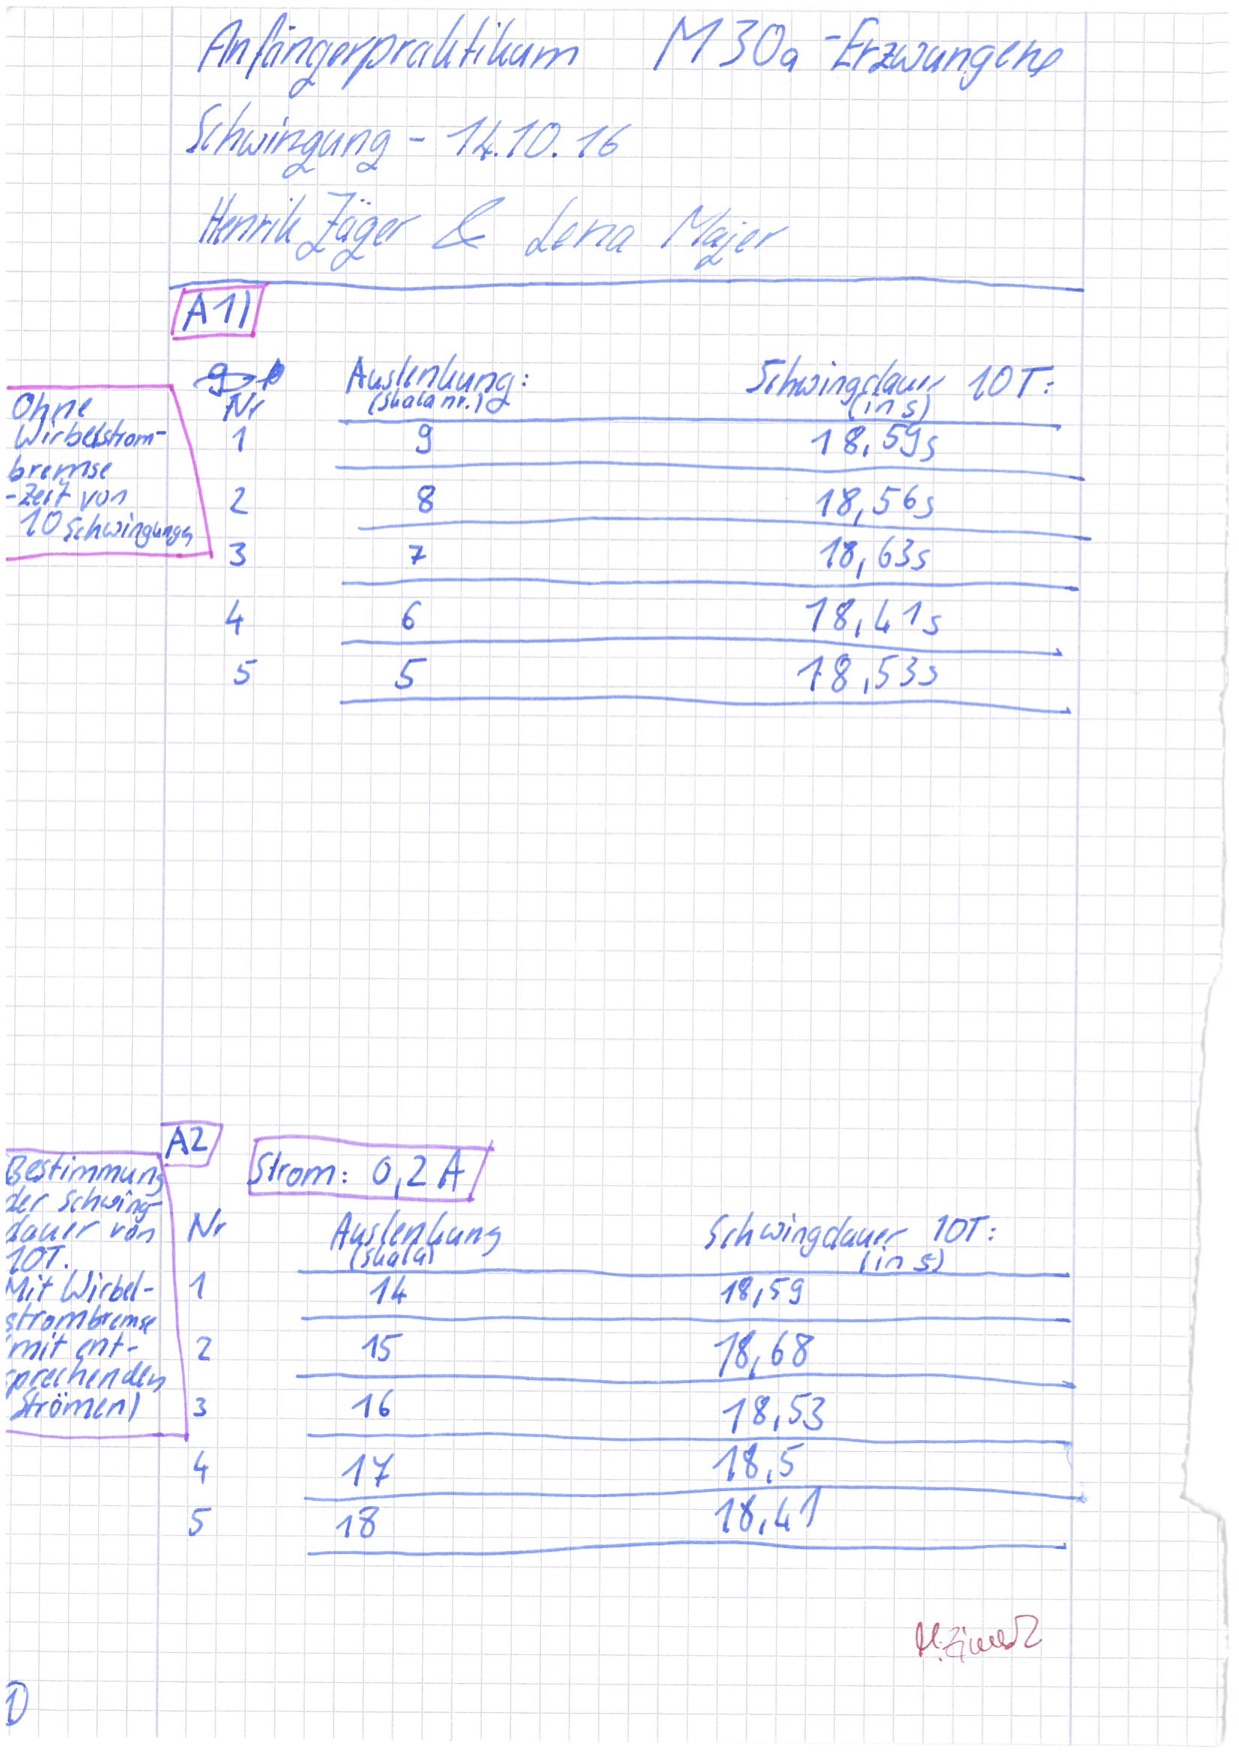
\includegraphics[scale=0.33]{1.jpg}
    	\captionof{figure}[]{Messprotokoll 1. Seite}
    	\pagebreak
    	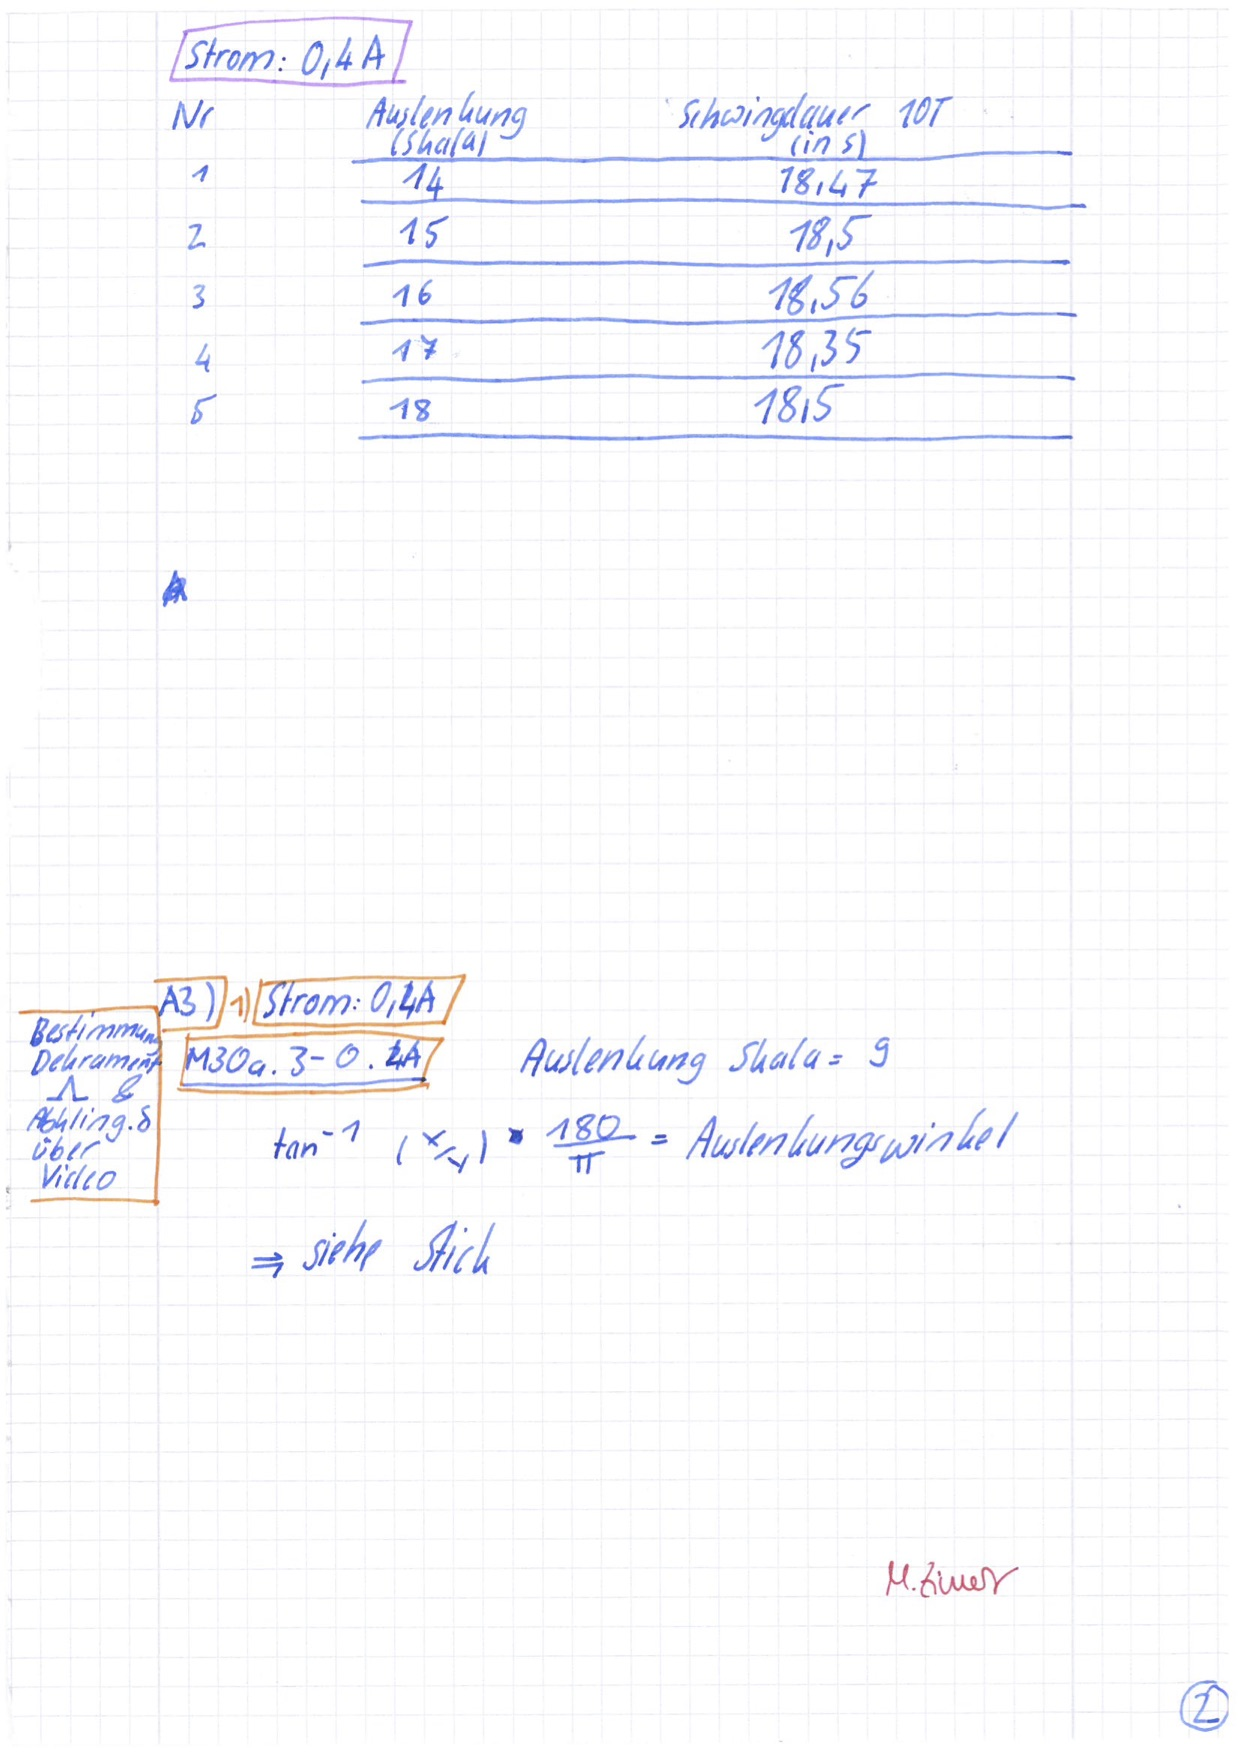
\includegraphics[scale=0.33]{2.jpg}
    	\captionof{figure}[]{Messprotokoll 2. Seite}
    	\pagebreak
    	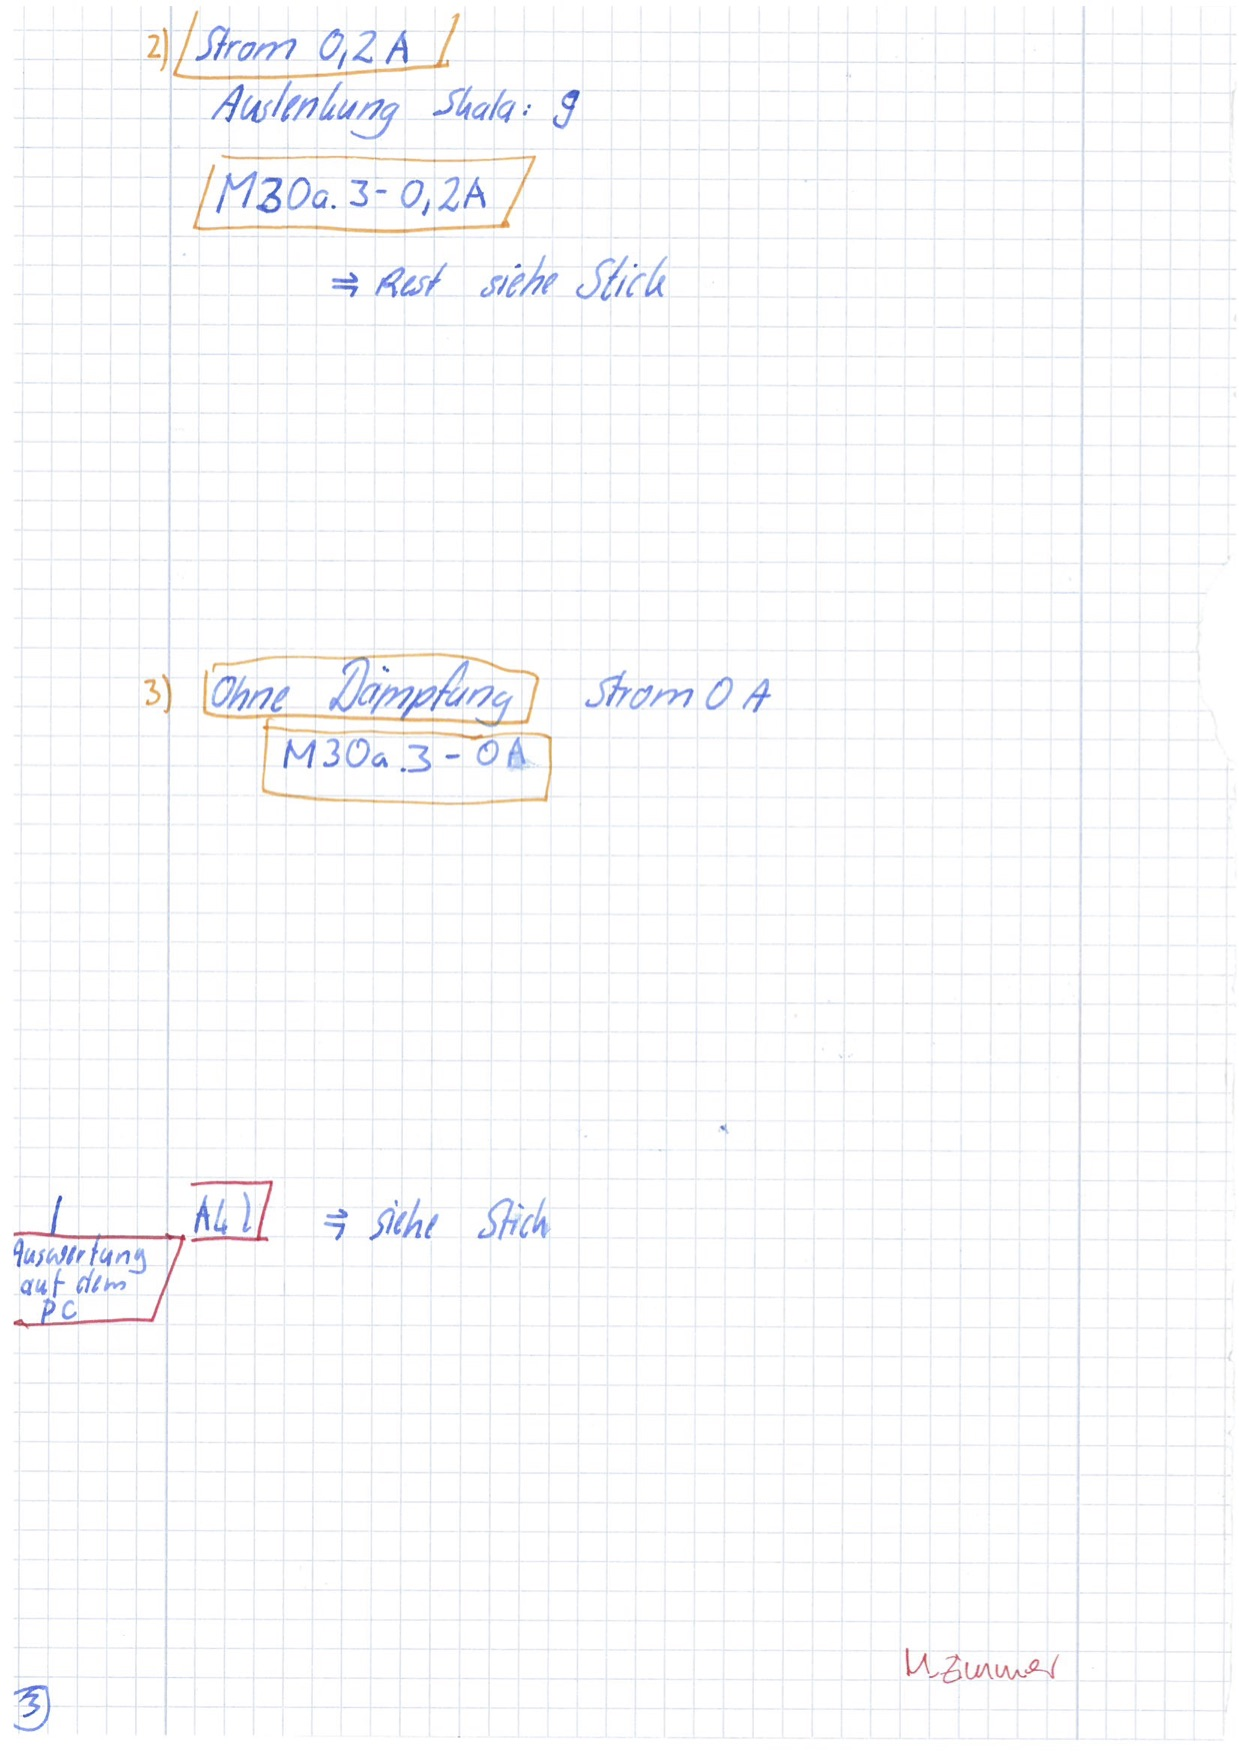
\includegraphics[scale=0.33]{3.jpg}
    	\captionof{figure}[]{Messprotokoll 3. Seite}
    	\pagebreak
    	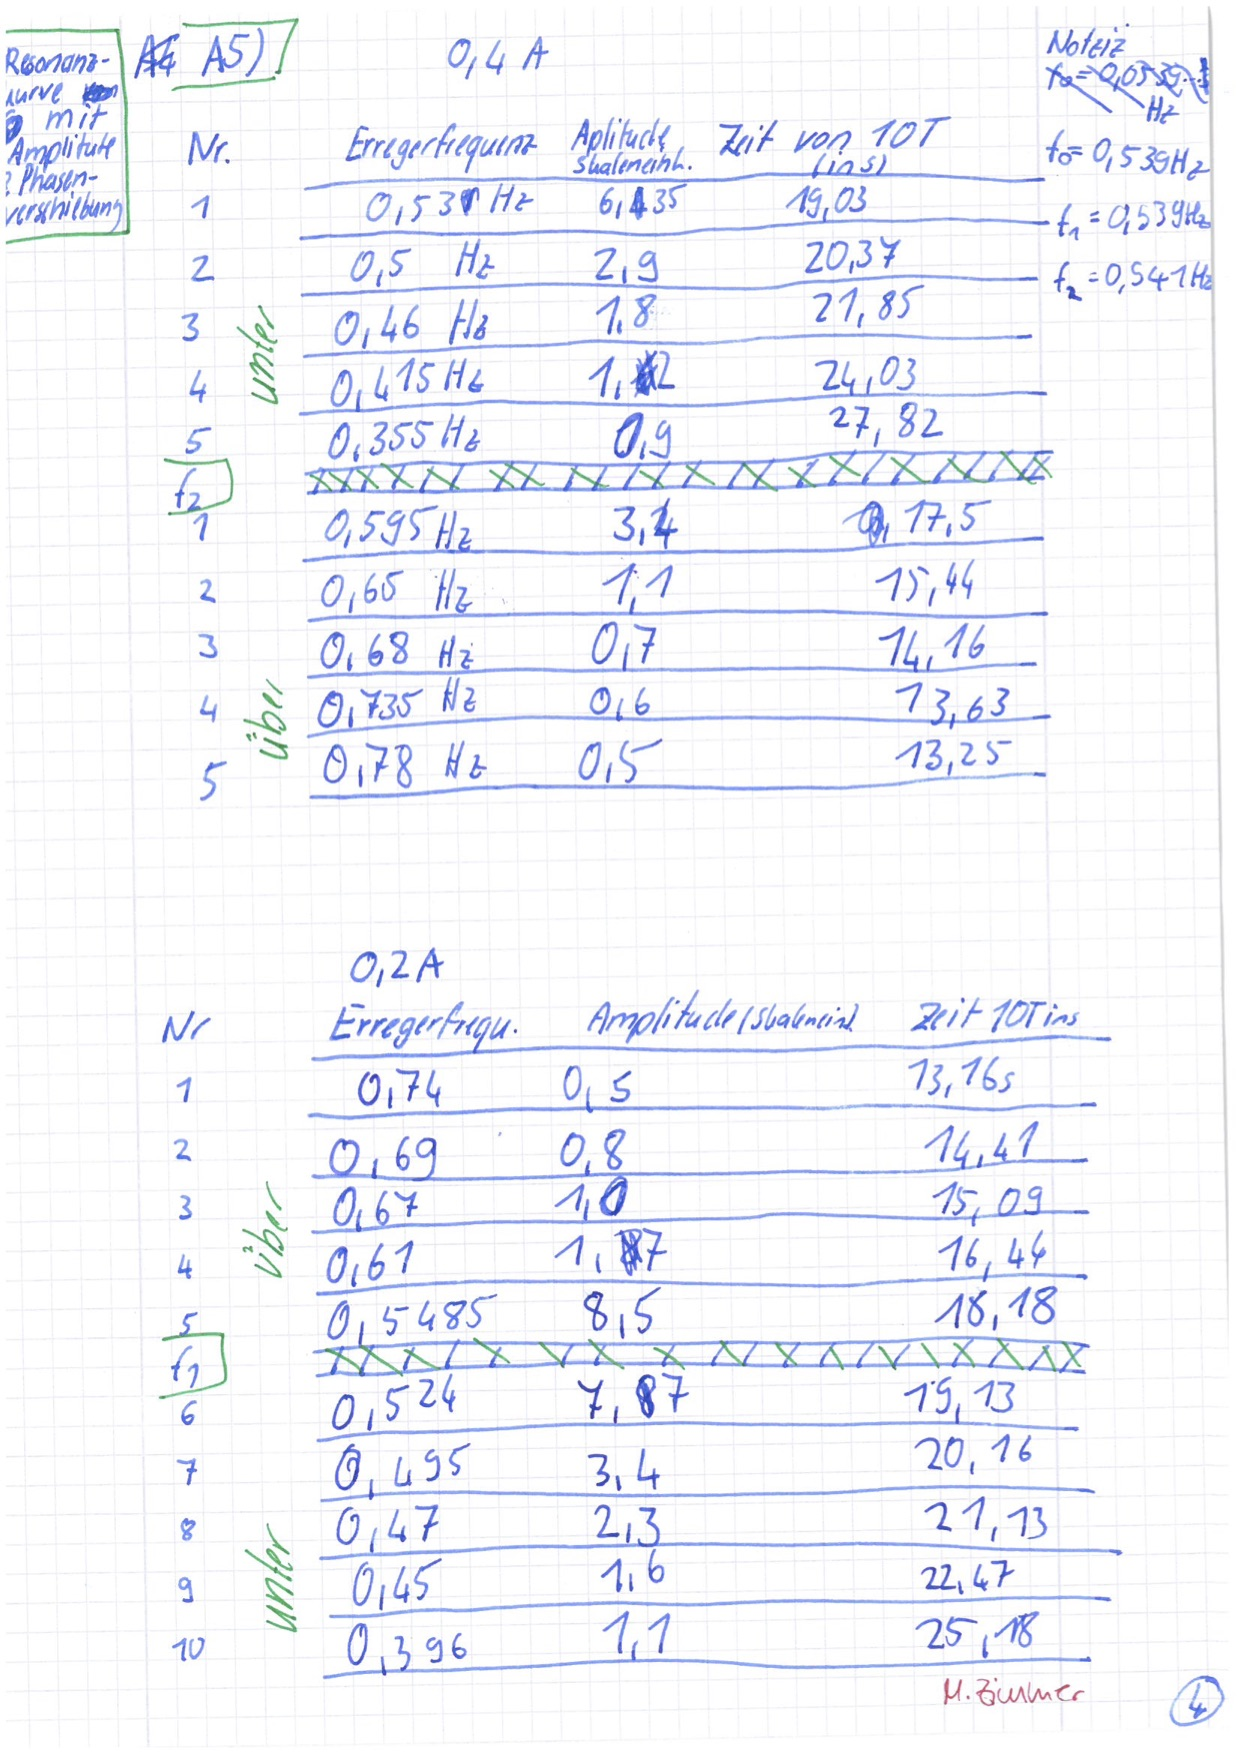
\includegraphics[scale=0.33]{4.jpg}
    	\captionof{figure}[]{Messprotokoll 4. Seite}
    	\pagebreak
    \end{center}
\end{document}
